\documentclass[a4paper, 12pt]{article}

\usepackage[utf8]{inputenc}
\usepackage[T1]{fontenc}
\usepackage{textcomp}
\usepackage{amssymb}
\usepackage{newtxtext} \usepackage{newtxmath}
\usepackage{xcolor}
\usepackage{tcolorbox}
\usepackage{expex}
\usepackage{forest}
\DeclareMathAlphabet{\mathcal}{OMS}{cmsy}{m}{n}
\usepackage{parskip}
\newcommand{\verbf}[1]{\textcolor{blue}{#1}}
\newcommand{\subjf}[1]{\underline{#1}}
\newcommand{\objf}[1]{\textcolor{red}{#1}}
\newcommand{\tensef}[1]{\colorbox{yellow}{#1}}
\newcommand{\noun}[1]{\textsc{#1}}
\newcommand{\adj}[1]{\textit{#1}}
\newcommand{\prep}[1]{\textcolor{purple}{#1}}
\usepackage{graphicx}

\begin{document}

    
Ce n'est pas souvent considéré, mais un des points critiques de la théorie
darwinienne est l'insubstantialité morale. Pour l'éthos chrétien, du moins
d'après l'interprétation traditionnelle, le bien et le mal sont des substances
actives. (La doctrine de la \textit{privatio boni}, indépendamment de ce que nous
pensons, est artificielle et tardive.) Mais, d'un point de vue métaphysique, le
monde darwinien est un monde insubstantiel, et notre manière de considérer
certaines choses comme bonnes ou mauvaises est un phénomène biologique que la
neuroscience moderne réduit, correctement à mon avis, au cerveau.

Je ne veux pas discuter de ces choses; je voudrais plutôt montrer comment Redon a
exprimé ces problèmes dans son œuvre. La raison est triple.

Premièrement, Redon étudia la théorie de l'évolution avec un certain degré de
détail. C'était un ami d'Armand Clavaud, un botaniste qui l'initia aux lectures
de Darwin et Lamarck, mais aussi à celles de Baudelaire, Poe, et certains poètes
hindous. Redon se fascina pour ce que l'on pourrait appeler le problème de
l'origine, et produisit un album magnifique nommé précisément \textit{Les
Origines}. En 1881, il vit à Paris une exposition des aborigènes captifs de
la Terre de Feu et dit:

\begin{quote}
They provided me with a dream of primitive life, nostalgia for the pure and
simple existence of our beginnings. I have never felt with as much force the gap
our own nature spans between the crawling beast and our higher destiny. . .
.What a poem, this quite perfect organism, emerging from the primeval slime to
stand beside us and stammer out the first stanzas of a universal hymn.
\end{quote}

\begin{figure}[htbp]
    \centering
    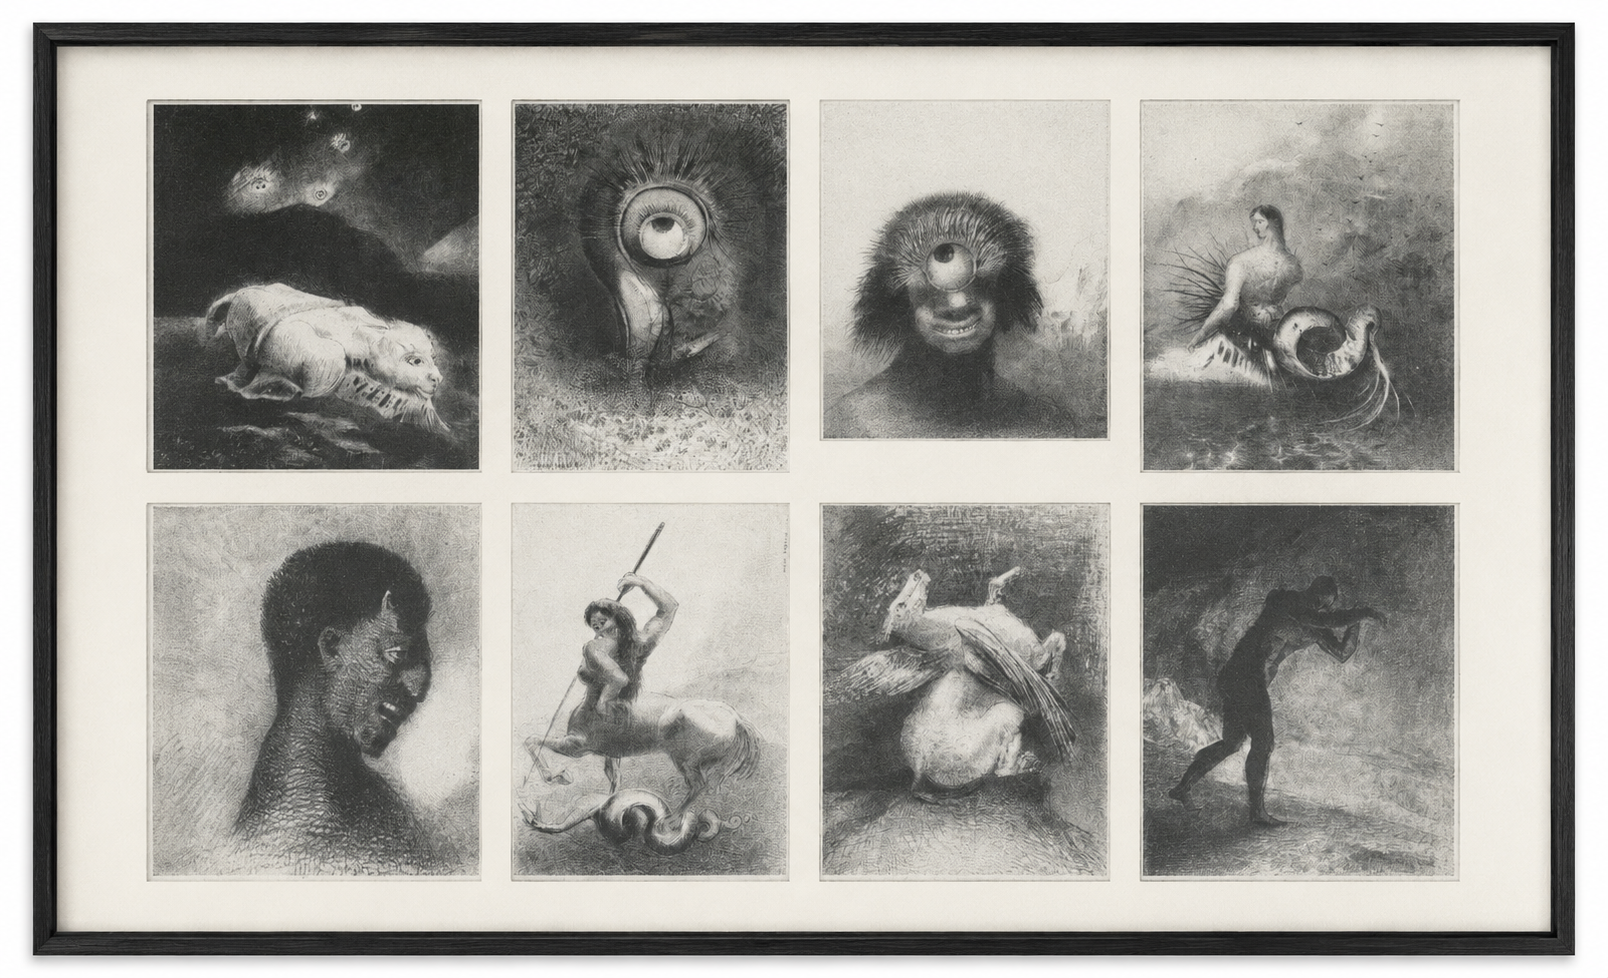
\includegraphics[width=\textwidth]{../Images/LesOrigens.png}
    \caption{Les Origines}
    \label{fig:lesorigens}
\end{figure}

Cette citation révèle sa fascination, bien que mélangée aux préjugés propres
de son temps, pour la «vase primitive» et l'histoire évolutive de l'homme.

Deuxièmement, Redon comprenait les problèmes posés par la théorie de l'évolution
de manière plus sophistiquée que ses contemporains. L'Européen moyen
s'inquiétait du passage d'une forme à une autre, un problème réel mais mineur
d'un point de vue scientifique et spirituel. La mesure dans laquelle l'Europe se
préoccupait de cette question se révèle dans les nombreuses caricatures
représentant des singes qui se transforment en hommes, satires qui au fil du
temps se transformèrent en satires d'elles-mêmes. Mais Redon était fasciné par
un problème plus fondamental et complexe; à savoir, le passage de l'informe à ce
qui a une forme. C'est le problème du xάος hésiodique, que Darwin ressuscita
et qui est plus difficile à résoudre et à caricaturer. Par exemple, dans \textit{Les
Origines} nous voyons l'œuvre \textit{Quand s'éveillait la vie au fond de la
matière obscure}, dans laquelle une créature est en train de surgir précisément d'une
vase primitive, tandis que, sur le fond obscur et depuis l'espace, des têtes
flottantes s'approchent de la Terre. D'après Sven Sandström, le premier expert à
organiser \textit{Les Origines}, la lecture de cette œuvre est temporelle: «When
the seed from space arrives on earth life starts in early states to develop from
matter."


\begin{figure}[H]
    \centering
    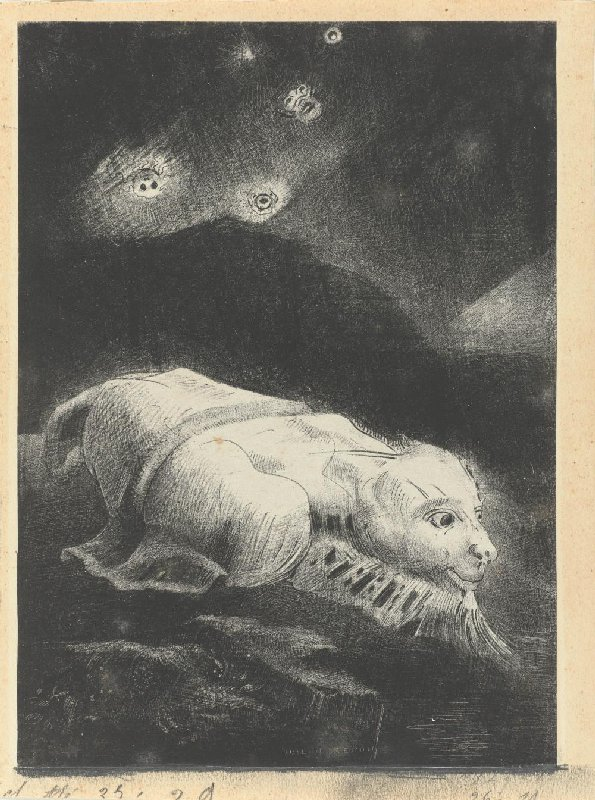
\includegraphics[width=\textwidth]{../Images/Redon2.jpg}
    \caption{Quand s'éveillait la vie au fond de la matière obscure}
    \label{fig:redon2}
\end{figure}

Il y a un autre example dans l'œuvre \textit{ Le Polype difforme flottait sur
les rivages, sorte de cyclope souriant et hideux}, aussi de \textit{Les
Origines}, dans laquelle nous voyons une «polype» (le mot fait référence à
Polyphème). La créature n'est ni animal ni homme. Ses traits grotesques évoquent
le primitif et ce qui n'a pas encore de forme, mais qui est en train de
l'acquérir. Mais, comme une étude a indiqué [1], le «polype» est aussi 


\begin{quote}


«... un organisme unicellulaire qui faisait l'objet de nombreuses investigations
scientifiques à l'époque, non seulement en tant que l'une des premières formes
de vie, mais aussi parce qu'il était étrangement inclassable. Ni tout à
fait plante, ni tout à fait animal, il fut désigné par les naturalistes comme un
emblème de l'informe et de l'indéterminisme»

\end{quote}



\begin{figure}[H]
    \centering
    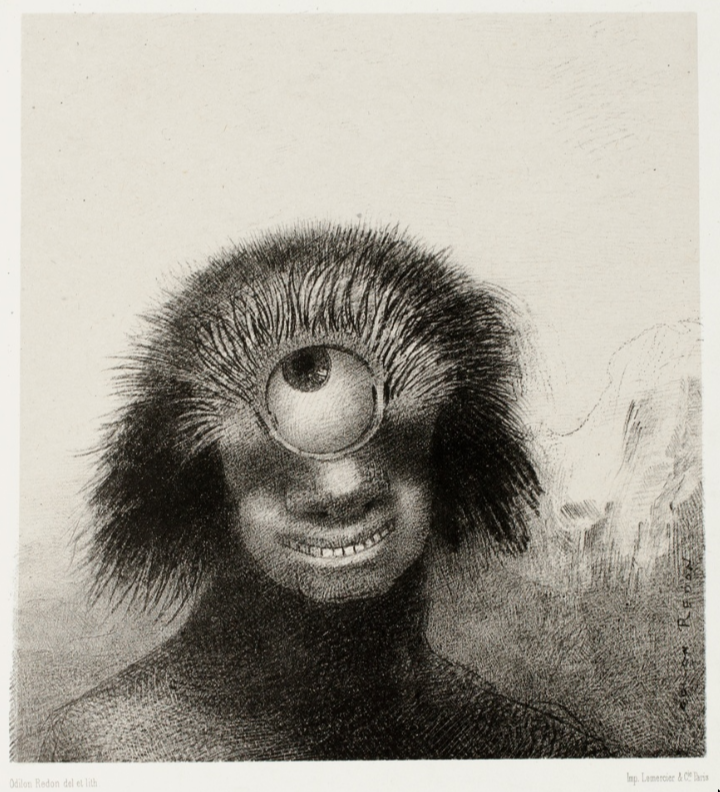
\includegraphics[width=\textwidth]{../Images/Redon4.png}
    \caption{Le Polype difforme flottait sur les rivages, sorte de cyclope souriant et hideux}
    \label{fig:redon2}
\end{figure}

Finalement, malgré sa compréhension de la théorie de l'évolution et son désir
d'imaginer le passage de l'informe à la complexité de la vie comme quelque chose
de matériel, Redon pressentait une force spirituelle sous-jacente à la vie. Il a
même dit, dans ses \textit{Confidences d'Artiste}, qu'Armand Clavaud était un
admirateur fervent de Spinoza, et il n'est pas difficile d'imaginer que Redon le
lisait aussi. Il dessina un Christ, mais appela l'œuvre \textit{Buda}, en
suggérant que toutes les religions émanent d'une source commune. Bien qu'immergé
dans le cercle symboliste ---il était habitué des réunions de Mallarmé---, son
intérêt scientifique lui fit comprendre comme aucun autre les principes
spinozistes qui sous-tendent la théorie du double aspect. Tandis que la plupart
des symbolistes pressentaient dans la réalité sensible un secret esthétique soit
merveilleux, soit décadent, Redon voyait un arcane spirituel qui non seulement
ne contredisait pas la science, mais la sublimait.

\begin{figure}[H]
    \centering
    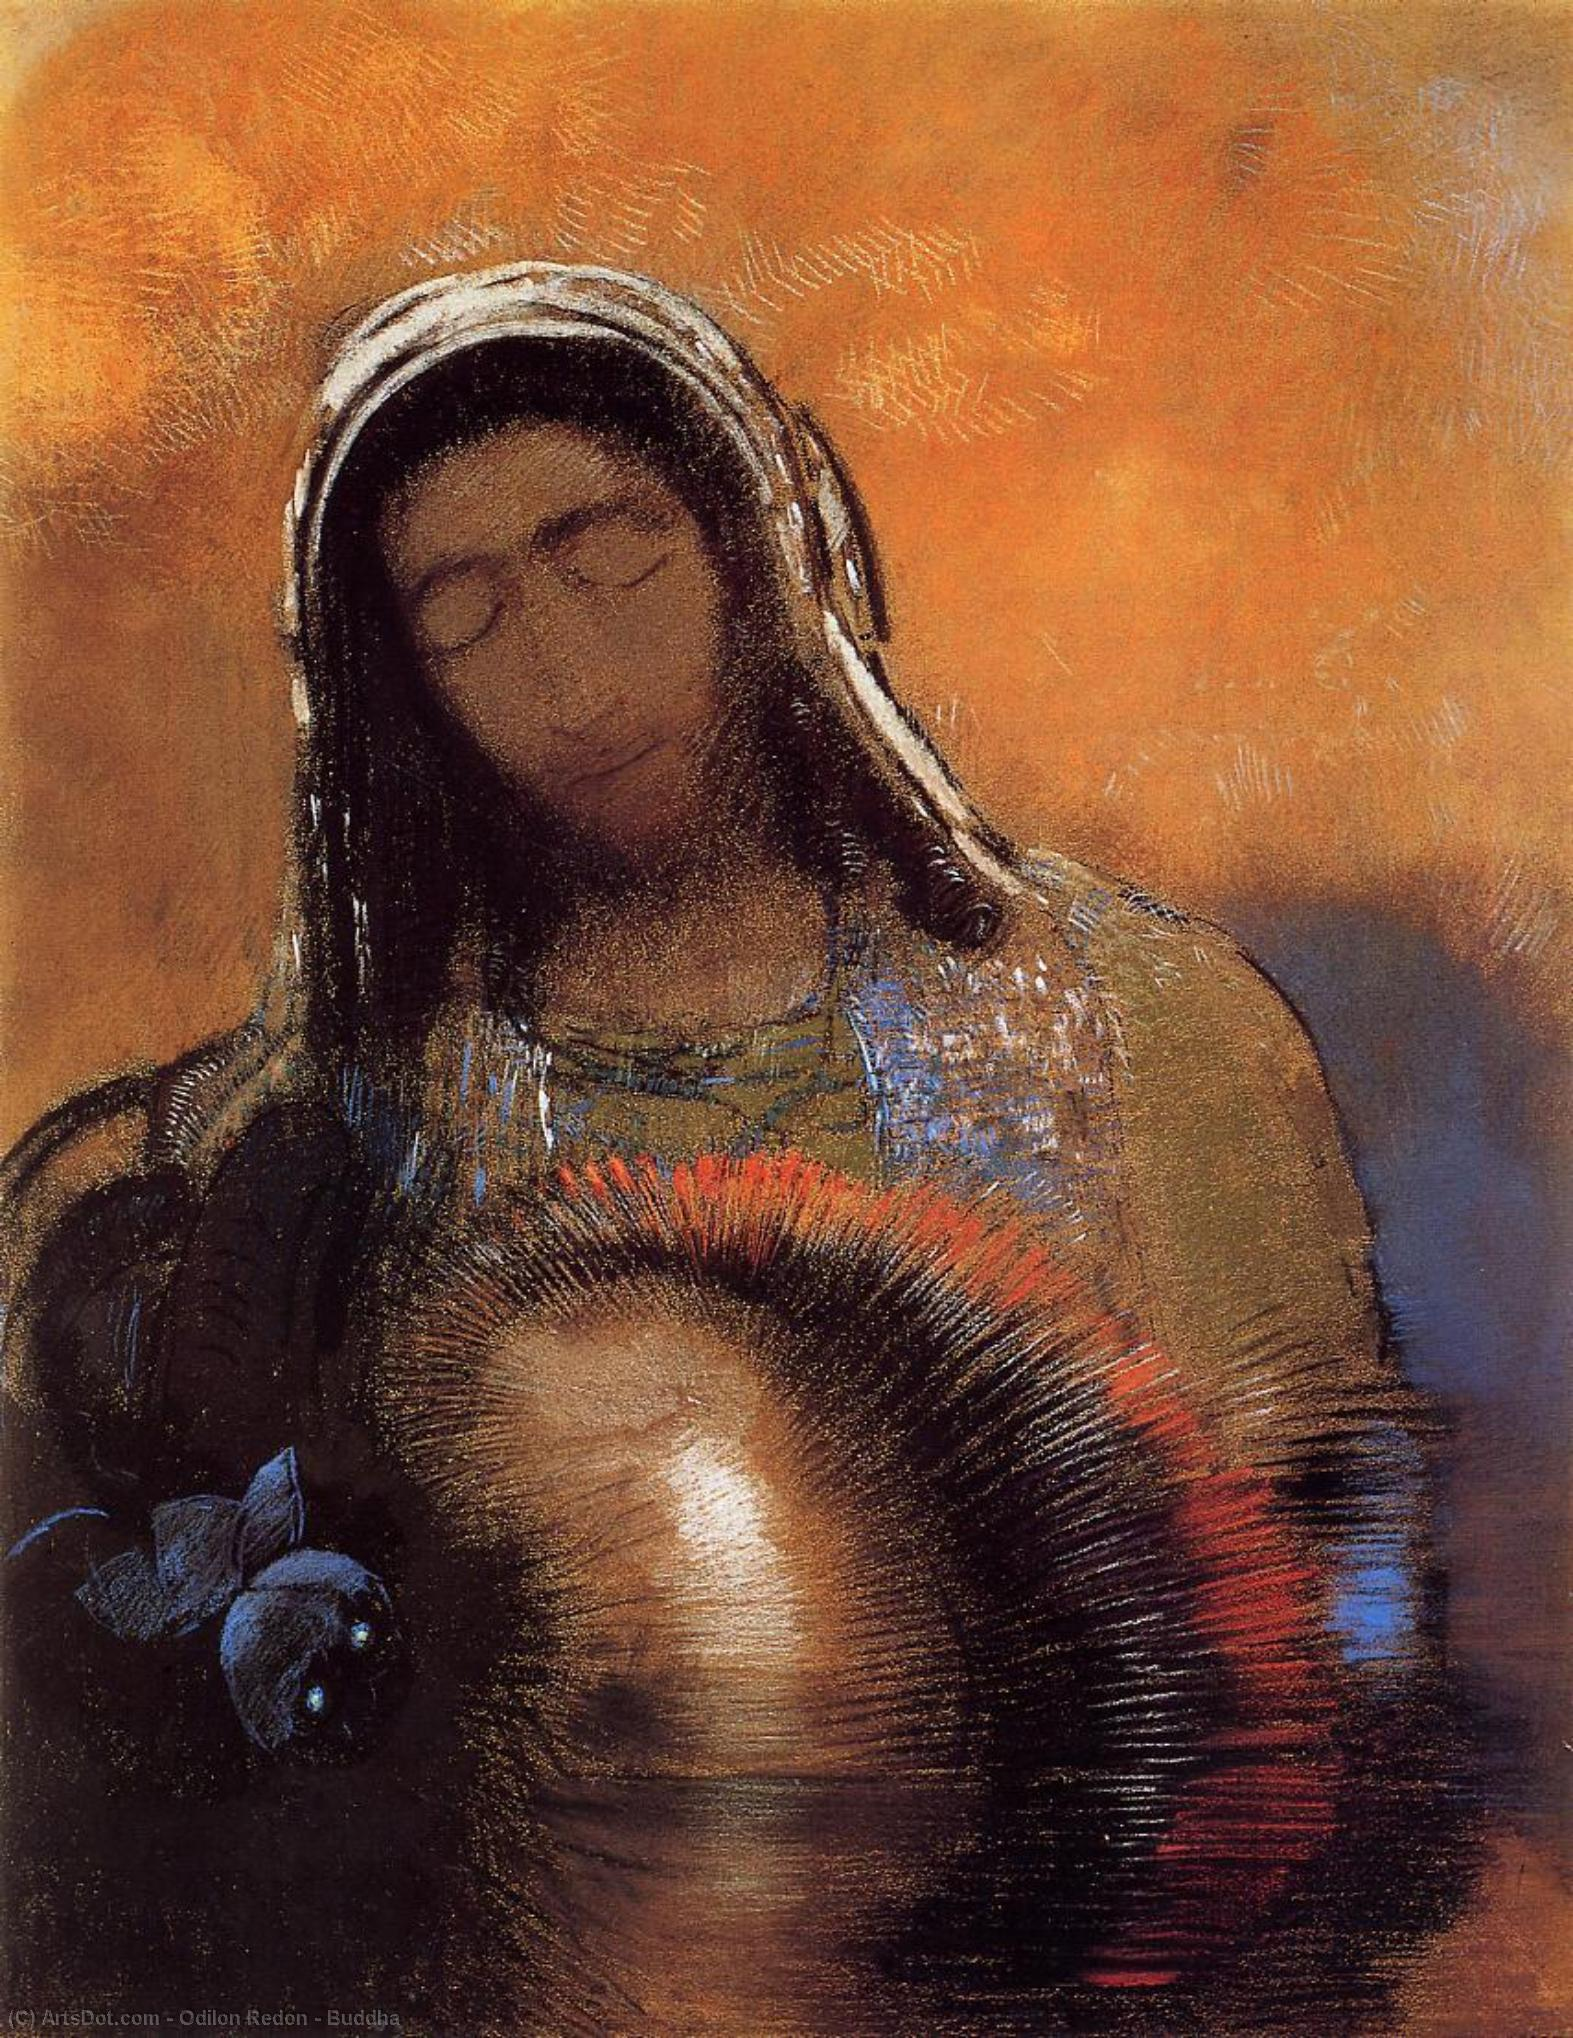
\includegraphics[width=\textwidth]{../Images/Redon3.jpeg}
    \caption{Buda}
    \label{fig:redon2}
\end{figure}

La vision de la science de Redon était \textit{correcte} au sens usuel du terme:
à savoir, elle est en accord avec mes jugements et préjugés. Blague à part, la
vision spinoziste du monde est, il me semble, la seule possible face à tout ce
que nous avons appris de la neuroscience. Comme c'est souvent le cas, l'art
surpasse la science pour exprimer la nature des choses. La plupart des
références à Redon en ligne le décrivent comme un fou, comme un homme qui
coloria des visions étranges et inexplicables. Mais il ne fit rien de plus que
se poser les bonnes questions face aux découvertes de son temps et les sublimer
avec un art exquis.

Je voudrais commenter un dernier aspect de l'art de Redon. Jusqu'ici, j'ai parlé
de Redon comme quelqu'un qui comprit certains problèmes propres à son époque et les
exprima avec une imagination et une sensibilité particulières. Mais je n'ai rien
dit à propos du problème de l'insubstantialité morale : j'ai seulement raisonné
sur le problème de l'origine, et j'ai suggéré vaguement une ontologie spinoziste
comme solution à l'apparent vide ouvert par Darwin et la science en général
[[2]]. Quelle que soit la réponse que Redon trouva au problème moral, nous
l'ignorons; mais dans une de ses dernières œuvres je comprends qu'il en a trouvé
une. Car le plus grand signe de richesse morale et spirituelle est la capacité
de comprendre le mal avec compassion et tendresse, et c'est précisément ce que
Redon montre dans l'huile \textit{Le Cyclope}.

Dans \textit{Le Cyclope}, Redon explore le motif classique du cyclope Polyphème
et son amour pour Galatée. Bien qu'Ovide, dans le livre XIII des
\textit{Métamorphoses}, ait su décrire «cette créature impitoyable, terrifiante
même pour les forêts, que nul étranger n'a jamais croisée impunément», avec
une certaine tendresse, la plupart des représentations de Polyphème dans l'art
sont bestiales et impies. Elles représentent le monstre, la brute, l'idiot.
Redon est l'un des rares qui devina dans l'amour de Polyphème une force si
tendre, si pure, si innocente, qui constituait peut-être une qualité rédemptrice.
Dans \textit{Le Cyclope} nous voyons Polyphème en train de garder Galatée alors
qu'elle dort. Son visage, bien que bizarre, est aimable et tranquille. Il la
voit comme quelqu'un qui surveille le sommeil d'un être cher. Et tout arrive dans une
scène champêtre et pacifique, où les couleurs ---choisies dans le style typique du
Redon tardif--- transmettent un bonheur paisible.

C'est suffisant. J'espère avoir montré deux choses. D'un côté, que Redon n'était pas
un fou qui coloriait des fantaisies inexplicables, mais un artiste profondément
intéressé par l'idée d'exprimer certains problèmes posés par le darwinisme et la science
de son temps. De l'autre, que son intérêt pour la science non seulement ne l'a
empêché de poursuivre avec une forme chrétienne et singulière de symbolisme, mais
que ce mélange dotait son art d'une originalité et d'une pitié sublimes.







\end{document}



